\section{Architettura di sistema }
\subsection{Modello architetturale}
Il sistema è stato progettato seguendo l'\textbf{architettura esagonale}, un modello che mira alla separazione tra business logic dell'applicazione e i servizi esterni, le fonti dati e le interfacce utente. Questa struttura pone il core\textsubscript{G} al centro, circondato da ports\textsubscript{G} che fungono da interfaccia tra il core\textsubscript{G} e il mondo esterno.

Il \textbf{core\textsubscript{G}} dell'applicazione è il fulcro del sistema, che contiene la logica di dominio e le regole di business. La sua progettazione punta ad evitare riferimenti diretti a dettagli tecnologici specifici, promuovendo l'indipendenza dal contesto esterno.

Le \textbf{ports\textsubscript{G}} costituiscono il confine tra il core\textsubscript{G} dell'applicazione e l'esterno, garantendo una comunicazione strutturata. Esistono due tipi di ports\textsubscript{G}: 
\begin{itemize}
    \item Inbound Port (o Use Case): per le invocazioni del core\textsubscript{G} da parte di componenti esterni, attraverso un'interfaccia definita. Sono in pratica dei punti di accesso al core\textsubscript{G} e isolano la logica di dominio da implementazioni specifiche;
    \item Outbound Port: consentono al core\textsubscript{G} di accedere a funzionalità esterne (e.g. interazione con librerie esterne\textsubscript{G} o sistemi di persistenza). Mettono a disposizione un'astrazione che preserva l'indipendenza del core\textsubscript{G} dai dettagli tecnici specifici. 
\end{itemize}

I \textbf{services\textsubscript{G}} costituiscono il livello più esterno dell'applicazione, fanno parte della business logic. L'implementazione dei services\textsubscript{G} si concentra sulla logica di dominio, senza preoccuparsi degli aspetti tencologici specifici.

Gli \textbf{adapters\textsubscript{G}} formano il livello più esterno dell'applicazione. Esistono due tipi di adapters\textsubscript{G}: 
\begin{itemize}
    \item Input Adapters\textsubscript{G} (o Controllers): invocano operazioni sulle Inbound Port, traducendo le azioni provenienti dall'esterno in chiamate alle ports\textsubscript{G} in ingresso al core\textsubscript{G}, rendendo le richieste esterne comprensibili per il core\textsubscript{G};
    \item Output Adapters\textsubscript{G}: invocano operazioni sulle Outbound Port, traducendo le azioni del core\textsubscript{G} in operazioni comprensibili per il mondo esterno.
\end{itemize}

\begin{figure}[H]
    \centering
    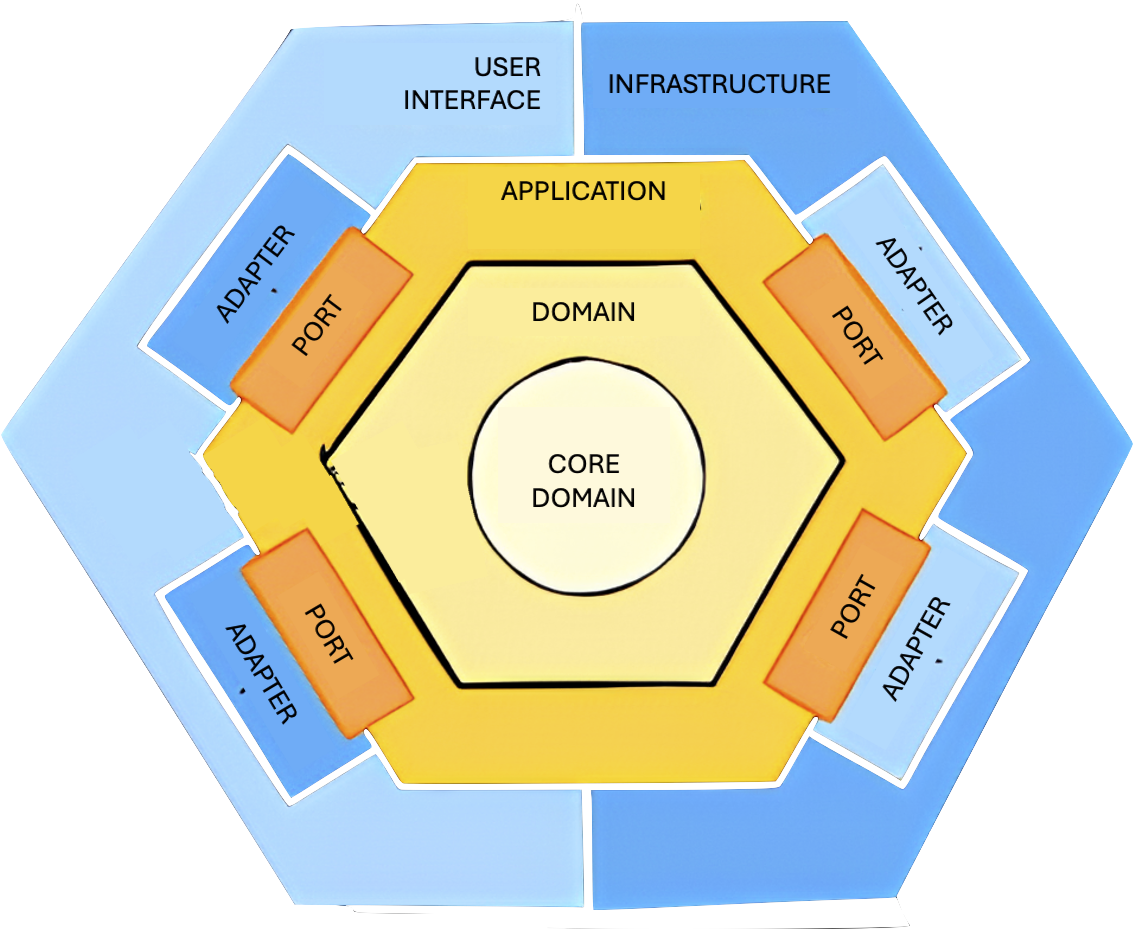
\includegraphics[width=0.5\textwidth]{images/HEX.png}
    \caption{Rappresentazione dell'architettura esagonale}
    \label{fig:architettura}
\end{figure}

\subsection{Componenti}
L'architettura del sistema è suddivisa in:
\begin{itemize}
    \item Frontend: si occupa di fornire un'interfaccia grafica all'utente per interagire col sistema. Inoltra le domande dell'utente al backend e visualizza i risultati;
    \item Backend: si occupa di elaborare le richieste degli utenti, interagendo con il sistema di persistenza e i servizi esterni, in particolare dialoga con il database vettoriale e con gli LLM;
    \item Database: è responsabile della memorizzazione della documentazione per la RAG e delle chat con relativi messaggi.
\end{itemize}
\subsubsection{Assemblaggio delle componenti}
Le componenti sono assemblate tramite Docker Compose, per facilitare l'esecuzione e la gestione di più container docker. 
In particolare sono stati prodotti i seguenti container:
\begin{itemize}
    \item pgvector: espone l'istanza del database sulla porta 5432, permettendo al backend di accedere ai relativi dati;
    \item app: espone la componente di backend sulla porta 5001, dando al frontend la possibilità di accedere ai servizi offerti;
    \item frontend: espone l'applicazione web sulla porta 4200, dando la possibilità all'utente di connettersi e interagire col sistema;
    \item data processing: responsabile dello scraping, dell'indicizzazione e salvataggio nel DB.
\end{itemize}
\subsection{Struttura del sistema}
\subsubsection{Frontend}
\subsubsubsection{Introduzione}
L'approccio adottato per lo sviluppo del front-end\textsubscript{G} si basa su una combinazione flessibile di pattern e pratiche tipiche del framework Angular\textsubscript{G}, senza aderire rigidamente a un unico schema architetturale come MVC\textsubscript{G} o MVVM\textsubscript{G}. Questa scelta consente di bilanciare modularità, scalabilità e semplicità nella gestione dello stato, adattandosi alle specifiche esigenze del progetto. 
\newline \newline La struttura dell'applicazione si articola in due aree funzionali ben distinte (utente e amministrativa), basate su componenti standalone\textsubscript{G} — come SidebarComponent, ChatboxComponent e AppComponent per l'area utente; AdminLoginComponent e AdminDashboardComponent per l'area amministrativa — supportati da servizi dedicati quali ApiService e ChatService. I componenti sono responsabili della presentazione, mentre i servizi gestiscono la comunicazione con il back-end\textsubscript{G} tramite API RESTful\textsubscript{G} (nel caso di ApiService) e centralizzano la logica di business e lo stato (come in ChatService). 
\newline \newline In questo modo, operazioni quali la creazione di conversazioni, l'invio di messaggi o la gestione dei feedback vengono delegate ai servizi, rendendo i componenti più leggeri e riutilizzabili. La gestione dello stato è un elemento chiave dell'architettura: l'introduzione di un servizio come ChatService, che utilizza il pattern Observer\textsubscript{G} tramite BehaviorSubject\textsubscript{G} di RxJS\textsubscript{G} per centralizzare conversazioni, messaggi e conversazione attiva, consente ai componenti di reagire dinamicamente ai cambiamenti attraverso gli observable. Questo garantisce un'interfaccia utente\textsubscript{G} reattiva e fluida, resa possibile grazie a strumenti asincroni come async/await\textsubscript{G} e firstValueFrom\textsubscript{G}.
\newline \newline La sicurezza è gestita attraverso meccanismi appropriati al contesto: sessioni utente anonime persistenti tramite localStorage\textsubscript{G} per l'area chat, e autenticazione basata su hash SHA-256\textsubscript{G} con token JWT\textsubscript{G} per l'area amministrativa, implementata tramite interceptor HTTP\textsubscript{G}.
\subsubsubsection{Design Pattern}
L'applicazione front-end implementa specifici pattern di progettazione software che ne definiscono l'architettura complessiva. La scelta di questi pattern si allinea con le best practice di Angular e con le esigenze progettuali.
\subsubsubsubsection{Pattern Creazionali}
\begin{itemize}
    \item Singleton
    \newline\newline L'intero sistema di dependency injection\textsubscript{G} di Angular implementa implicitamente questo pattern. Tutti i servizi (ApiService e ChatService) sono dichiarati con @Injectable{providedIn: 'root'}, garantendo un'unica istanza per l'intera applicazione. Grazie a questo sistema si riesce la centralizzazione dello stato dell'applicazione, la prevenzione di inconsistenze e l'ottimizzazione delle risorse attraverso il riuso delle istanze di servizio. 
\end{itemize}
\subsubsubsubsection{Pattern Strutturali}
\begin{itemize}
    \item Decorator
    \newline\newline Si usa il sistema nativo di decoratori TypeScript/Angular\textsubscript{G} (@Component, @Injectable, @Input e @Output) per estendere dinamicamente il comportamento delle classi e di AuthInterceptor per decorare le richieste HTTP. Così facendo si separano le responsabilità e si riutilizza il codice.
    \item Façade
    \newline\newline ApiService astrae le complessità delle chiamate HTTP e ChatService nasconde i dettagli implementativi della gestione delle conversazioni. Il vantaggio è il disaccoppiamento tra logica di business e interfaccia utente. 
\end{itemize}
\subsubsubsubsection{Pattern Comportamentali}
\begin{itemize}
    \item Observer
    \newline\newline Uso estensivo di BehaviorSubject e Observable di RxJS per gestire flussi di dati asincroni e aggiornamenti dell'interfaccia utente. 
    \item Mediator
    \newline\newline AppComponent funge da mediatore per la comunicazione tra componenti figli come SidebarComponent e ChatboxComponent. 
\end{itemize}
\subsubsubsection{Scenari}
Il front-end\textsubscript{G} presenta un’area pubblica e un’area riservata all’admin come richiesto dal capitolato\textsubscript{G}. La prima può essere utilizzata da un utente generico, e non è previsto un sistema di autenticazione\textsubscript{G}, mentre la seconda come si può intuire è riservata all’amministratore e sono richieste delle credenziali di accesso.
\subsubsubsubsection{Scenari Pubblici}
\begin{itemize}
    \item Inizializzazione: 
    \newline \newline Viene verificato se esista già una sessione\textsubscript{G} salvata nel localStorage\textsubscript{G} del dispositivo dal quale si intende usufruire dell’applicativo. Se esiste allora vengono recuperate le conversazioni con i rispettivi messaggi, altrimenti viene creata una nuova sessione di cui si tiene traccia tramite un ID di sessione generato in maniera univoca. Inoltre, nel caso di una sessione nuova viene generata una conversazione di default che permette all'utente di interagire con l'assistente digitale\textsubscript{G}. 
    \item Gestione Conversazioni:
    \begin{itemize}
        \item L'utente può aggiungere conversazioni tramite un pulsante dedicato, ed è previsto un limite di 10 conversazioni; 
        \item L'utente può selezionare una qualsiasi delle conversazioni presenti così recuperando lo storico di messaggi;
        \item L'utente puù eliminare qualsiasi conversazioni desideri, qualora eliminasse la conversazione attiva, al suo posto viene generata automaticamente una nuova conversazione. 
    \end{itemize}
     \item Gestione Messaggi:
     \begin{itemize}
         \item L'utente può inviare messaggi, con limite di 500 caratteri, per i quali è previsto un messaggio di risposta dall'assistente digitale;
         \item L'utente può valutare la qualità di risposta tramite un sistema di feedback\textsubscript{G} positivi e negativi visibili sotto ogni messaggio dell’assistente;
         \item I feedback inviati vengono registrati ma non possono essere modificati successivamente.
     \end{itemize}
\end{itemize}
\subsubsubsubsection{Scenari Admin}
\begin{itemize}
    \item Accesso:
    \newline \newline L'admin accede tramite un URL\textsubscript{G} dedicato (/admin) e vede la schermata di login\textsubscript{G}. Inserisce la password che viene trasformata in hash SHA-256 lato client prima di essere inviata al server. Con credenziali corrette, l'admin entra nel dashboard\textsubscript{G} (/admin/dashboard), altrimenti riceve un messaggio di errore. I tentativi di accesso non autorizzati al dashboard vengono bloccati e reindirizzati al login attraverso un Guard Angular\textsubscript{G}.
    \item Funzionalità:
    \begin{itemize}
        \item Totale conversazioni;
        \item Totale feedback positivi;
        \item Totale feedback negativi;
        \item Tasso di soddisfazione.
    \end{itemize}
\end{itemize}
\subsubsubsection{Diagrammi delle Classi}
Seguendo la scia del paragrago precedente relativo agli scenari, l'analisi dei diagrammi delle classi\textsubscript{G} è ralazionato ai scenari pubblici e scenari admin. Ogni scenario sarà associato alle classi principali coinvolte e alle loro relazioni.
\subsubsubsubsection{Scenari Pubblici}
\begin{itemize}
    \item Inizializzazione
    \begin{itemize}
        \item Classi Coinvolte:
        \begin{itemize}
            \item AppComponent coordina l'inizializzazione dell'applicativo;
            \item SidebarComponent gestisce la lisa delle conversazioni;
            \item ChatboxComponent mostra la conversazione attiva e i relativi messaggi;
            \item ApiService gestisce le chiamate API RESTful\textsubscript{G} al back-end\textsubscript{G};
            \item ChatService gestisce lo stato delle conversazioni e dei messaggi.
        \end{itemize}
        \item Relazioni:
        \begin{itemize}
            \item AppComponent contiene SidebarComponent e ChatboxComponent come componenti figli;
            \item SidebarComponent e ChatboxComponent dipendonon da ChatService per accedere allo stato;
            \item ChatService usa ApiService per recuperare i dati iniziali dal back-end.
        \end{itemize}
    \end{itemize}
    \item Creazione di una Nuova Conversazione
    \begin{itemize}
        \item Classi Coinvolte:
        \begin{itemize}
            \item SidebarComponent contiene il pulsante per avviare la creazione;
            \item ChatService crea la conversazione e aggiorna lo stato;
            \item ApiService invial la richiesta HTTP al back-end per creare la conversazione.
        \end{itemize}
        \item Relazioni:
        \begin{itemize}
            \item ChatService invoca ApiService.createConversation() per la comunicazione con il back-end;
            \item ChatService notifica i componenti dell’aggiornamento tramite BehaviorSubject;
            \item AppComponent coordina la comunicazione tra SidebarComponent e ChatboxComponent tramite eventi (@Output) quando viene creata una nuova conversazione.
        \end{itemize}
    \end{itemize}
    \item Gestione Feedback
    \begin{itemize}
        \item Classi Coinvolte:
        \begin{itemize}
            \item ChatboxComponent visualizza e gestisce i pulsanti per i feedback;
            \item ChatService elabora e memorizza temporaneamente il feedback;
            \item ApiService invia il feedback al back-end.
        \end{itemize}
        \item Relazioni:
        \begin{itemize}
            \item ChatboxComponent invoca ChatService.sendFeedback() quando l’utente clicca un pulsante;
            \item ChatService invoca ApiService.sendFeedback() per inviare al backend.
        \end{itemize}
    \end{itemize}
\end{itemize}
\subsubsubsubsection{Scenari Admin}
\begin{itemize}
    \item Classi Coinvolte:
    \begin{itemize}
        \item AdminLoginComponent gestisce l'autenticazione;
        \item AdminDashboardComponent visualizza le statistiche;
        \item ApiService comunica con il backend;
        \item AuthInterceptor intercetta e modifica le richieste HTTP.
    \end{itemize}
    \item Relazioni:
    \begin{itemize}
        \item AdminLoginComponent usa ApiService per l’autenticazione;
        \item AdminDashboardComp usa ApiService per recuperare statistiche;
        \item AuthInterceptor aggiunge token alle richieste admin.
    \end{itemize}
\end{itemize}
\newpage
\subsubsection{Backend}
 Il sistema è architettato secondo il pattern esagonale (Ports and Adapters), dove il Core costituisce il dominio centrale dell'applicazione. Questa componente rappresenta il nucleo del sistema, caratterizzato da un isolamento completo dalle dipendenze esterne. Al suo interno sono contenute le regole di business fondamentali e le entità che definiscono i concetti chiave del dominio: le conversazioni, i messaggi e le sessioni. Il Core opera come un'unità autonoma, implementando la logica di business in modo indipendente dalle modalità di input/output dei dati.
\newline La comunicazione tra il Core e l'ambiente esterno è gestita attraverso le Porte, che definiscono le interfacce di interazione. Queste costituiscono i contratti formali attraverso i quali il Core stabilisce le modalità di comunicazione desiderate, astraendosi dalle implementazioni concrete. Le Porte rappresentano le specifiche tecniche che definiscono come il Core intende interagire con l'esterno, delegando la responsabilità dell'implementazione alle componenti periferiche.
\newline Il sistema è completato dagli Adattatori, che formano un layer periferico attorno al Core. Questi componenti implementano le interfacce definite dalle Porte, fungendo da intermediari tra il Core e le risorse esterne. Gli Adattatori si occupano della traduzione dei dati e delle richieste tra il dominio e l'ambiente esterno, garantendo che il Core rimanga isolato dalle specifiche implementative delle interfacce esterne.
\subsubsubsection{Componenti}
\subsubsubsubsection{CORE - ConversationService}
Nel core del sistema, la classe \texttt{ConversationService} si occupa principalmente della gestione delle sessioni, delle conversazioni, dei messaggi e dei feedback.

\subsubsection*{Gestione delle Sessioni}
Il servizio offre diversi metodi per la gestione delle sessioni:
\begin{itemize}
    \item \texttt{createSession()} permette di creare una nuova sessione.
    \item \texttt{readSession(sessionId)} recupera una sessione esistente dato un identificativo specifico.
    \item \texttt{updateSession(sessionId)} consente di aggiornare il timestamp di una sessione.
\end{itemize}

\subsubsection*{Gestione delle Conversazioni}
Per quanto riguarda le conversazioni, il servizio gestisce:
\begin{itemize}
    \item \texttt{createConversation(sessionId)} crea una nuova conversazione associata a una sessione esistente.
    \item \texttt{readConversations(sessionId)} restituisce tutte le conversazioni relative a una sessione specifica.
    \item \texttt{readConversationById(conversationId)} permette di recuperare una conversazione in base al suo ID.
    \item \texttt{deleteConversation(conversationId)} consente di eliminare una conversazione (o marcarla come eliminata).
    \item \texttt{updateConversationTimestamp(conversationId)} aggiorna il timestamp di una conversazione.
\end{itemize}

\subsubsection*{Gestione dei Messaggi}
Il sistema offre anche funzionalità per la gestione dei messaggi all’interno delle conversazioni:
\begin{itemize}
    \item \texttt{addMessage(conversationId, sender, content)} consente di aggiungere un nuovo messaggio a una conversazione esistente.
    \item \texttt{readMessages(conversationId)} restituisce tutti i messaggi di una determinata conversazione.
\end{itemize}

\subsubsection*{Gestione dei Feedback}
Infine, la gestione dei feedback si articola in diversi metodi:
\begin{itemize}
    \item \texttt{readFeedback(messageId)} recupera il feedback associato a un messaggio specifico.
    \item \texttt{addFeedback(messageId, feedback, content)} permette di aggiungere un feedback a un messaggio esistente.
    \item \texttt{readNumPositiveFeedback()} e \texttt{readNumNegativeFeedback()} forniscono il conteggio dei feedback positivi e negativi.
    \item \texttt{readFeedbackWithComments()} recupera tutti i feedback che contengono anche dei commenti.
\end{itemize}

\subsubsubsubsection{ADAPTER - DBRepository}
Gli adattatori sono responsabili della comunicazione tra il core del sistema e il database. In particolare, \texttt{DBRepository} si occupa dell'esecuzione delle query SQL e della gestione dei risultati:
\begin{itemize}
    \item \texttt{executeQuery(query, params)} esegue una query SQL passando i parametri necessari.
    \item \texttt{fetchOne(query, params)} recupera un singolo risultato dalla query.
    \item \texttt{fetchAll(query, params)} restituisce tutti i risultati di una query.
    \item \texttt{close()} chiude la connessione al database.
\end{itemize}



\subsubsubsubsection{ADAPTER - ContextExtractorService}
Il \texttt{ContextExtractorService} ha il compito di individuare i prodotti e le porzioni di documentazione (chunk) presenti nel database che risultano più pertinenti e coerenti con il prompt fornito dall'utente.\\ Il processo di ricerca \`e stato diviso in 2 macro-operazioni:
\begin{enumerate}
    \item Ricerca prodotti pi\`u coerenti;
    \item Ricerca chunk pi\`u coerenti, tra quelli che appartengono ai prodotti selezionati.
\end{enumerate}
All'interno del file \texttt{ContextExtractorService.py} ci sono delle costanti che possono essere modificate per ``scalare" la soluzione (ad esempio, avendo a disposizione pi\`u potenza di calcolo):
\begin{enumerate}
    \item \texttt{SIMILARITY\_THRESHOLD} \`e la soglia sotto la quale un prodotto non viene considerato;
    \item \texttt{TOP\_SIMILAR\_CHUNKS} \`e il numero di chunk che vengono inseriti come contesto del prompt;
    \item \texttt{TOP\_PRODUCTS\_FINAL} \`e il numero di prodotti ``coerenti" dai quali documenti saranno estratti i \texttt{TOP\_SIMILAR\_CHUNKS}.
\end{enumerate}
\texttt{ContextExtractorService} contiene i seguenti metodi:
\begin{itemize}
    \item \texttt{processUserInput(userInput)} \`e il metodo principale della classe e orchestra l'estrazione dei dati coerenti dal Database.\\ \texttt{userInput} \`e il testo del prompt fatto dall'utente.
    \item \texttt{getStructuredProducts()} estrae dal Database le informazioni riguardanti id, titolo, descrizione di ogni prodotto, insieme a 3 vettori che rappresentano rispettivamente l'informazione di ``id prodotto", ``id e titolo prodotto" e ``id, titolo e descrizione prodotto".
    \item \texttt{findTopNSimilarProducts(prodList, promptVector, n)} trova gli \texttt{n} prodotti pi\`u simili al prompt, utilizzando i vettori sopra citati.
    \item \texttt{aggregateSimilarities(similarProducts)} aggrega le informazioni estratte da \texttt{findTopNSimilarProducts}, in questo modo per ogni prodotto si avr\`a un unico punteggio di similarit\`a.
    \item \texttt{selectChunksEmbeddings(chunks, aggregatedSimilarProduct)} seleziona i chunk dei documenti associati ai prodotti pi\`u simili, restituendo i vettori di embedding per il confronto.
    \item \texttt{findTopNSimilar(chunksEmbeddings, userEmbeddings, n)} trova gli \texttt{n} chunk pi\`u simili rispetto al prompt utente confrontando gli embedding tramite similarit\`a coseno.
    \item \texttt{extractEtim()} estrae dal Database l'informazione relativa agli ETIM (dati tecnici) dei prodotti.
    \item \texttt{selectEtim(etim, textsToEmbed)} associa le informazioni ETIM ai chunk selezionati come contesto, restituendo un dizionario che mappa gli identificativi di prodotto ai relativi codici ETIM.
    \item \texttt{getEmbedding(prompt)} utilizza il modello di embedding \texttt{mxbai-embed-large} per generare un vettore di embedding a partire dal testo del prompt.
    \item \texttt{getDocumentsByProductId(productId)} recupera dal Database i documenti associati a un determinato prodotto, includendo il titolo del prodotto e il titolo del documento.
    \item \texttt{loadChunks()} estrae dal Database tutti i chunk di documentazione, inclusi gli embedding associati, per consentire la ricerca di contenuti pertinenti.
\end{itemize}
\subsubsubsubsection{ADAPTER - LLMResponseService}
Il \texttt{LLMResponseService} ha il compito di interfacciarsi con un modello di linguaggio per ottenere una risposta contestualizzata basata su una conversazione in corso, una domanda utente e un insieme di informazioni di contesto estratte dal Database.
Negli attributi della classe \`e possibile configurare il modello di linguaggio, il default \`e \texttt{llama3.1:8b}.
\texttt{LLMResponseService} contiene il seguente metodo:
\begin{itemize}
    \item \texttt{getLlmResponse(conversationPile, question, textsToEmbed, etimToEmbed)} si occupa di formattare i messaggi della conversazione, aggregare il contesto rilevante e inviare la richiesta al modello LLM per ottenere una risposta.
\begin{figure}[H]
    \centering
    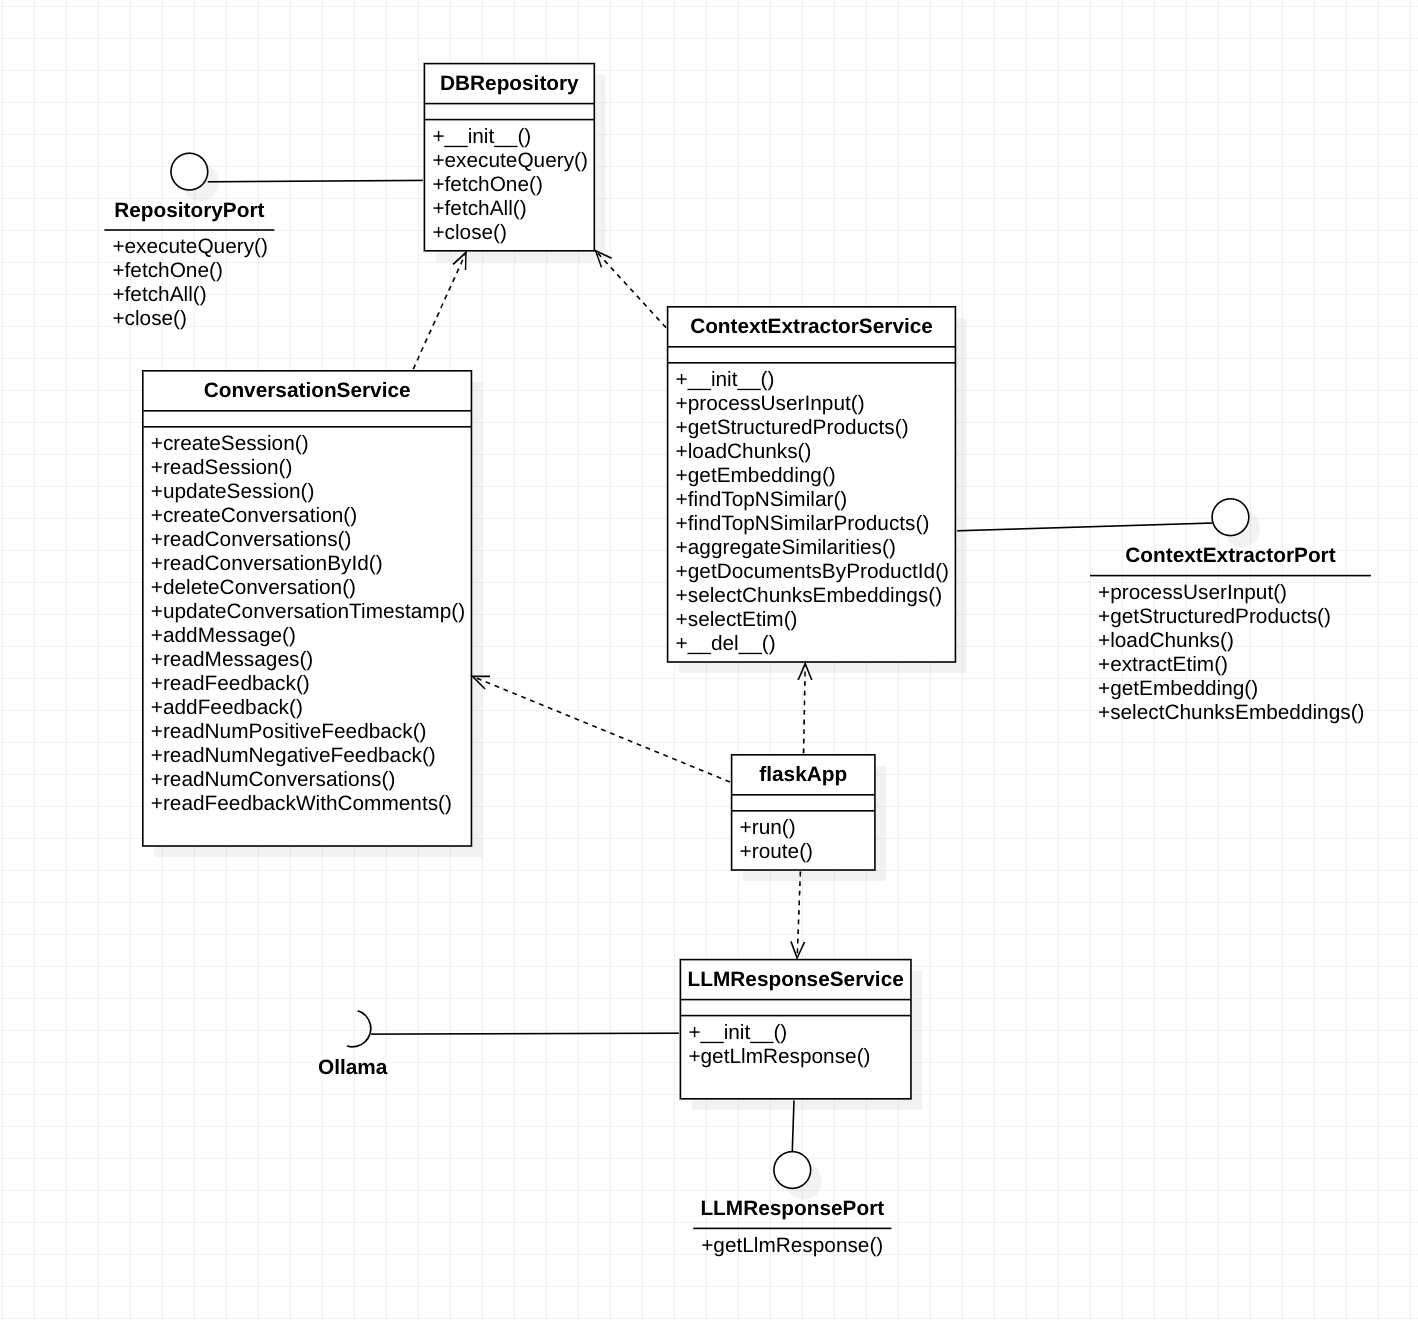
\includegraphics[width=\textwidth]{images/BackendUML.png}
    \caption{Schema delle classi utilizzate nel backend}
    \label{fig:architettura}
\end{figure}

\end{itemize}

\subsubsubsubsection{API - APIController}
Gli adattatori includono anche \texttt{APIController}, che gestisce gli endpoint delle API esposte dal sistema. Esistono vari endpoint per ciascuna delle operazioni descritte, a partire da quelli di test:
\begin{itemize}
    \item \texttt{testApi()} che consente di verificare il funzionamento generale del sistema.
\end{itemize}

\subsubsection*{Gestione delle Sessioni}
\begin{itemize}
    \item \texttt{apiCreateSession()} per creare una nuova sessione.
    \item \texttt{apiUpdateSession(sessionId)} per aggiornare una sessione esistente.
\end{itemize}

\subsubsection*{Gestione delle Conversazioni}
\begin{itemize}
    \item \texttt{apiCreateConversation()} per creare una conversazione.
    \item \texttt{apiReadConversations()} per ottenere tutte le conversazioni di una sessione.
    \item \texttt{apiReadConversationById(conversationId)} per ottenere una conversazione specifica.
    \item \texttt{apiDeleteConversation(conversationId)} per eliminare una conversazione.
    \item \texttt{apiUpdateConversationTimestamp(conversationId)} per aggiornare il timestamp della conversazione.
\end{itemize}

\subsubsection*{Gestione dei Messaggi}
\begin{itemize}
    \item \texttt{apiAddMessage()} per aggiungere un nuovo messaggio.
    \item \texttt{apiReadMessages()} per recuperare i messaggi di una conversazione.
\end{itemize}

\subsubsection*{Gestione dei Feedback}
\begin{itemize}
    \item \texttt{apiReadFeedbackByMessageId(messageId)} recupera il feedback associato a un messaggio.
    \item \texttt{apiAddFeedback()} permette di aggiungere un feedback.
\end{itemize}

\subsubsection*{Gestione della Dashboard}
\begin{itemize}
    \item \texttt{apiReadNumPositiveFeedback()} e \texttt{apiReadNumNegativeFeedback()} per ottenere il numero di feedback positivi e negativi.
    \item \texttt{apiReadNumConversations()} per conoscere il numero totale di conversazioni.
    \item \texttt{apiReadFeedbackWithComments()} per ottenere feedback che includono commenti.
\end{itemize}

Gli endpoint sono protetti da un sistema di sicurezza, con il decoratore \texttt{requireAPIKey(f)} che garantisce l’autenticazione tramite chiave API. Inoltre, la configurazione di CORS permette di gestire le richieste provenienti dal frontend.

\subsubsection{Database}
\begin{figure}[H]
    \centering
    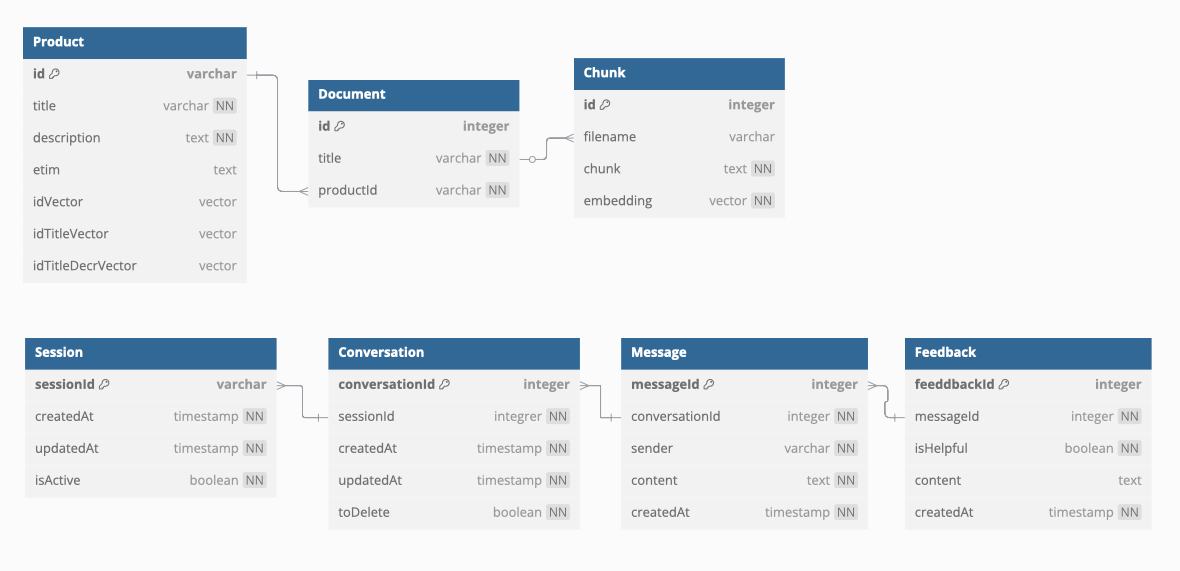
\includegraphics[width=\textwidth]{images/DB.png}
    \caption{Modello Entit\`a-Relazione}
    \label{fig:Diagramma ER}
\end{figure}

Nel database relazionale sono presenti sette tabelle per la persistenza delle informazioni da utilizzare nella RAG e delle conversazioni degli utenti.
\newline
Per quanto riguarda i dati relativi ai prodotti da utilizzare nelle fasi di ricerca del contesto per il modello di linguaggio ci sono tre tabelle di seguito descritte.
\begin{itemize}
    \item \textbf{Product}: immagazzina le informazioni primarie prelative ai prodotti disponibili nel sito web
    \begin{itemize}
        \item id: l'id del prodotto, in formato testuale;
        \item title: il titolo o nome del prodotto;
        \item description: la breve descrizione del prodotto presente nella pagina web dedicata;
        \item etim: i dati tecnici del prodotto presenti nella pagina web dedicata, sottoforma di stringa ("key: value;") a causa della variabilità dei dati disponibili a seconda del tipo di prodotto;
        \item idVector: la vettorizzazione dell'id del prodotto per le ricerche;
        \item idTitleVector: la vettorizzazione dell'id insieme al titolo del prodotto per le ricerche;
        \item idTitleDescrVector: la vettorizzazione dell'insieme di id, titolo e descrizione del prodotto per le ricerche.
    \end{itemize}
    \item \textbf{Document}: immagazzina le informazioni dei documenti estratti dalle pagine web dei prodotti
     \begin{itemize}
        \item id: id univoco;
        \item title: il titolo del documento;
        \item productId: l'id del prodotto a cui fa riferimento.
    \end{itemize}
    \item \textbf{Chunk}: immagazzina le informazioni dei chunk creati a partire dai documenti
     \begin{itemize}
        \item id: id univoco;
        \item filename: il titolo del documento da cui è stato estratto il chunk;
        \item chunk: il testo del chunk;
        \item embedding: la vettorizzazione del chunk per le ricerche.
    \end{itemize} 
\end{itemize}
Per quanto riguarda invece il salvataggio e la permanenza delle conversazioni degli utenti vengono usate quattro tabelle di seguito descritte.
\begin{itemize}
    \item \textbf{Session}: contiene le sessioni, ovvero le connessioni degli utenti
    \begin{itemize}
        \item sessionId: id univoco che identifica la sessione dell'utente;
        \item createdAt: data e ora della creazione della sessione;
        \item updatedAt: data e ora dell'ultima modifica alla sessione;
        \item isActive: valore booleano che indica se la sessione sia ancora attiva o meno, di default a true, diventa automaticamente false dopo 30 giorni di inattività.
    \end{itemize} 
    \item \textbf{Conversation}: contiene le conversazioni degli utenti
    \begin{itemize}
        \item conversationId: id univoco;
        \item sessionId: id della sessione a cui appartiene;
        \item createdAt: data e ora della creazione della conversazione;
        \item updatedAt: data e ora dell'ultima modifica alla conversazione;
        \item toDelete: valore booleano che indica se la conversazione vada eliminata o meno, può diventare true su scelta dell'utente o allo scadere della sessione associata.
    \end{itemize} 
    \item \textbf{Message}: contiene tutti i messaggi inviati sia dagli utenti che dal modello LLM
    \begin{itemize}
        \item messageId: id univoco;
        \item conversationId: id della conversazioen a cui appartiene;
        \item sender: indica se il messaggio è stato inviato dall'utente o è una risposta del modello;
        \item content: il contenuto del messaggio stesso;
        \item createdAt: data e ora della creazione del messaggio.
    \end{itemize} 
    \item \textbf{Feedback}: contiene i feedback lasciati dagli utenti
    \begin{itemize}
        \item feedbakcId: id univoco;
        \item messageId: id del messaggio su cui è stato creato il feedback;
        \item isHelpful: booleano, indica un feedback positivo o negativo;
        \item content: il contenuto del feedback qualora l'utente desiderasse lasciarlo;
        \item createdAt: data e ora della creazione del feedback.
    \end{itemize} 
\end{itemize}


\subsubsection{Elaborazione dei Dati}
Una  componente essenziale per il funzionamento del prodotto è la raccolta dei dati dal sito web di Vimar e la loro elaborazione e salvataggio nel database. Queste attività sono ad opera del container  \texttt{dataProcessing} al cui avvio parte lo scraping del sito web che salva i dati dei prodotti in un file json. Successivamente lo stesso file è il punto di partenza per l'elaborazione dei dati e la generazione dei chunk a partire dai documenti associati ai prodotti, infine vi è il salvataggio nel database.  
Nel dettaglio:
\begin{itemize}
\item \texttt{productsElaboration.py} gestisce la manipolazione e l'analisi dei dati relativi ai prodotti, applicando eventuali filtri o trasformazioni;
\item \texttt{chunkElabotation.py} è particolarmente utile quando si lavora con grandi quantità di dati, poiché divide l'elaborazione in blocchi (chunk) per ottimizzare le prestazioni e ridurre il carico sulla memoria;
\item \texttt{embeddingLocal.py} è un modulo che si occupa della generazione di embedding locali,  utilizzati per analisi semantiche avanzate o per un sistema di raccomandazione basato su similarità tra prodotti:
\item \texttt{dataSaving.py} è il modulo che si occupa del salvataggio dei dati nel database.
\end{itemize}

L'esecuzione di questo container, che può richiedere diversi minuti, anche ore per la generazione dei chunck, si conclude dopo il salvataggio dei dati nel database.

\begin{figure}[H]
    \centering
    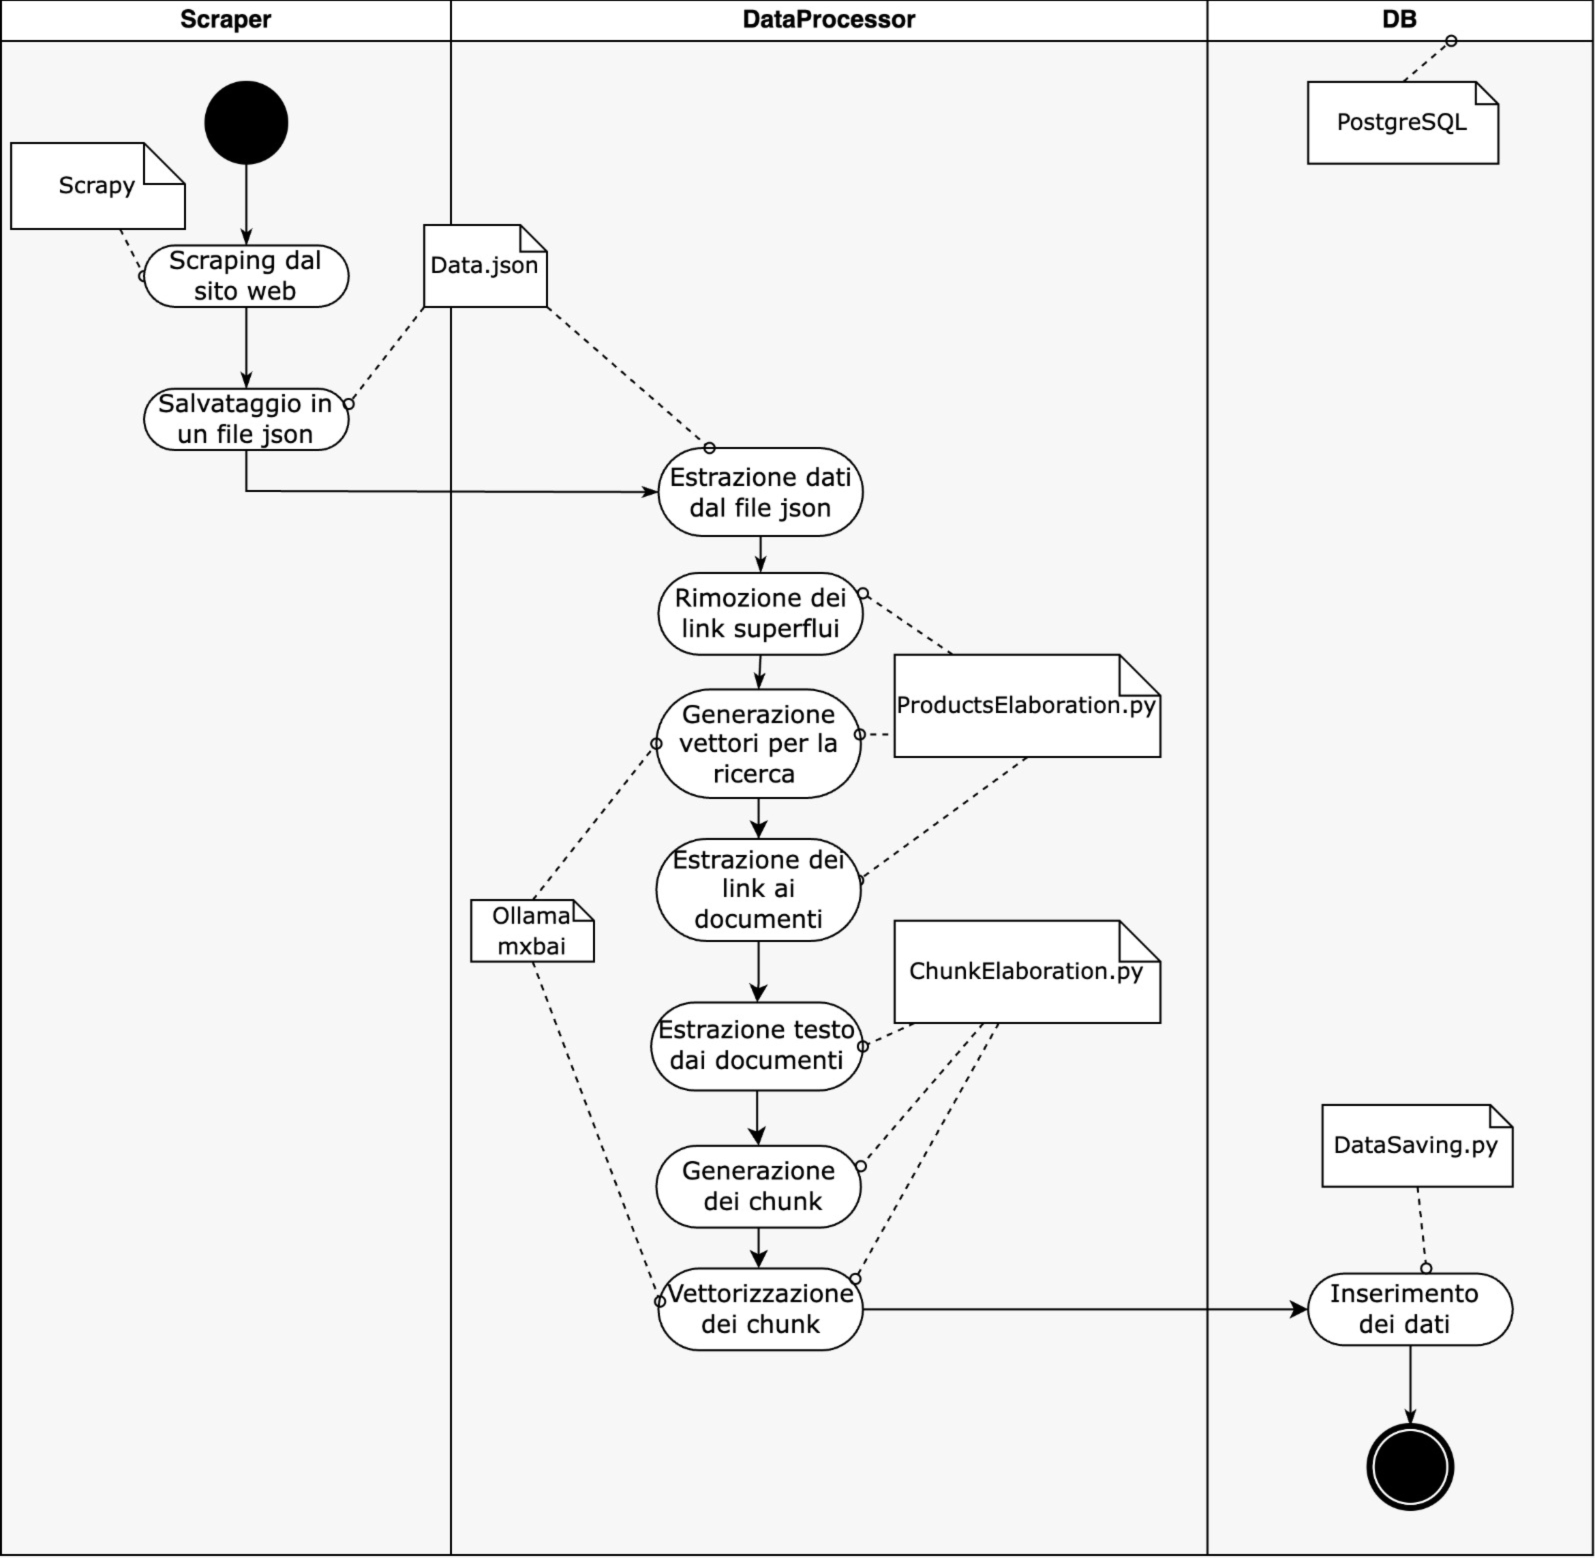
\includegraphics[width=\textwidth]{images/flussoSalvataggioDati.png}
    \caption{Diagramma delle attivit\`a del flusso di Elaborazione Dati}
    \label{fig:architettura}
\end{figure}


\subsubsection{ Dipendenze e Tecnologie Utilizzate}
L’elenco delle dipendenze è definito nel file requirements.txt, che include una serie di librerie fondamentali per il funzionamento del sistema:

\begin{itemize}
    
\item Flask per la gestione del server web tramite API.

\item Ollama per l’elaborazione del linguaggio naturale,  utilizzato per l'analisi dei testi associati ai prodotti.

\item PostgreSQL come database relazionale, scelto per la sua affidabilità e capacità di gestione di grandi volumi di dati.

\item Librerie per la manipolazione e l'analisi dei dati, come numpy e scikit-learn.

\item pypdf, che indica la funzionalità legata all'elaborazione di documenti PDF.

\end{itemize}